\subsection{Pictograms}
Pictograms are used in many places throughout the Giraf project.
A pictogram is an image which resembles an action or an object.
Pictograms are used in place of text since many on the citizens using the Giraf project is not able to read.
Two examples of pictograms are shown in~\myref{fig:pictograms}.

% https://en.wikibooks.org/wiki/LaTeX/Floats,_Figures_and_Captions#Subfloats
\begin{figure}[H]
    \centering
    \begin{subfigure}[b]{0.2\textwidth}
    	\fbox{
\includegraphics[width=\dimexpr\textwidth-2\fboxsep-2\fboxrule\relax]{figures/pictograms/pictogramsealion.png}}
        \caption{Sealion}
        \label{fig:sealion}
    \end{subfigure}
    \qquad
    \begin{subfigure}[b]{0.2\textwidth}
		\fbox{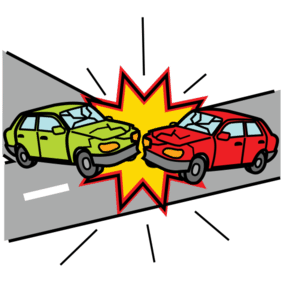
\includegraphics[width=\dimexpr\textwidth-2\fboxsep-2\fboxrule\relax]{figures/pictograms/pictogramtrafficcolision.png}}
        \caption{Traffic Collision}
        \label{fig:traffic_collision}
    \end{subfigure}
    \caption{Examples pictograms.}\label{fig:pictograms}
\end{figure}

Pictograms will often appear with an icon indicating something about them, these icons are called indicators.
This is to indicate what actions are available, pressing the pictogram will perform an action, such as a trash bin indicating that a deletion will happen when tapping the bin.
Two examples of this is shown in~\myref{fig:pictograms_with_indicators}

\begin{figure}[H]
    \centering
    \begin{subfigure}[b]{0.2\textwidth}
    	\fbox{
\includegraphics[width=\dimexpr\textwidth-2\fboxsep-2\fboxrule\relax]{figures/pictograms/pictogramsealion_with_indicator.png}}
        \caption{Sealion with wrench}
        \label{fig:sealion-with-wrench}
    \end{subfigure}
    \qquad
    \begin{subfigure}[b]{0.2\textwidth}
		\fbox{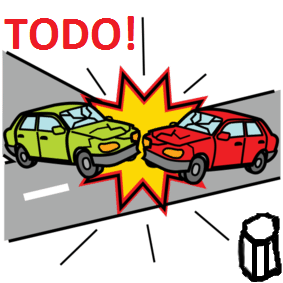
\includegraphics[width=\dimexpr\textwidth-2\fboxsep-2\fboxrule\relax]{figures/pictograms/pictogramtrafficcolisionn_with_indicator.png}}
        \caption{Traffic Collision with trash bin}
        \label{fig:trafficcollision-with-wrench}
    \end{subfigure}
    \caption{Examples pictograms with indicators.}\label{fig:pictograms_with_indicators}
\end{figure}